\documentclass[a4paper,fleqn]{cas-sc}
\bibliographystyle{unsrtnat}
\usepackage[sort&compress,numbers]{natbib}


%%%Author definitions
\def\tsc#1{\csdef{#1}{\textsc{\lowercase{#1}}\xspace}}
\tsc{WGM}
\tsc{QE}
\tsc{EP}
\tsc{PMS}
\tsc{BEC}
\tsc{DE}
%%%

% Uncomment and use as if needed
%\newtheorem{theorem}{Theorem}
%\newtheorem{lemma}[theorem]{Lemma}
%\newdefinition{rmk}{Remark}
%\newproof{pf}{Proof}
%\newproof{pot}{Proof of Theorem \ref{thm}}

\begin{document}
\let\WriteBookmarks\relax
\def\floatpagepagefraction{1}
\def\textpagefraction{.001}

% Short title
\shorttitle{}

% Short author
\shortauthors{Morales et~al.}

% Main title of the paper
\title [mode = title]{Optimal monitoring design for uncertainty quantification during geologic CO$_2$ sequestration: A machine learning approach}                      
% Title footnote mark eg: \tnotemark[1]

% First author
% Options: Use if required
% eg: \author[1,3]{Author Name}[type=editor,
%       style=chinese,
%       auid=000,
%       bioid=1,
%       prefix=Sir,
%       orcid=0000-0000-0000-0000,
%       facebook=<facebook id>,
%       twitter=<twitter id>,
%       linkedin=<linkedin id>,
%       gplus=<gplus id>]
\author[1,2]{Misael M. Morales}[]
\cormark[1]
\ead{misaelmorales@lanl.gov}
\credit{Conceptualization of this study, Methodology, Software, Writing - Original draft preparation}

% Second author
\author[1]{Mohamed Mehana}[]
\cormark[1]
\ead{mzm@lanl.gov}
\credit{Conceptualization, Writing, Funding acquisition}

% Third author
\author[1]{Bailian Chen}[]
\credit{Conceptualization, Software, Funding acquisition}

% Address/affiliation
\affiliation[1]{organization={Earth and Environmental Sciences Division, Los Alamos National Laboratory},
    city={Los Alamos},
    postcode={NM 87544}, 
    country={USA}}

% Address/affiliation
\affiliation[2]{organization={Hildebrand Department of Petroleum and Geosystems Engineering, The University of Texas at Austin}, 
    city={Austin},
    postcode={TX 78712},
    country={USA}}

% Corresponding author text
\cortext[cor1]{Corresponding author}

% Here goes the abstract
\begin{abstract}
Geologic CO$_2$ sequestration (GCS) projects have large uncertainties in geologic properties, and require optimal monitoring designs for risk assessment and management. An effective monitoring design is crucial to ensure the safe and permanent geologic storage of CO$_2$. Optimal monitoring design involve an optimal placement of monitoring wells, and optimal monitoring measurement data (pressure, CO$_2$ saturation, temperature, etc.). We have developed a filtering-based data assimilation approach to design an optimal GCS monitoring strategy for well placement and monitoring data design. To efficiently solve the optimization problem and reduce computational costs, Artificial Neural Networks are used to develop computationally efficient reduced-order models based on full-physics numerical simulations of CO$_2$ injection in saline aquifers. We demonstrate our approach in two scenarios of CO$_2$ leakage through legacy or abandoned wellbores where an optimal monitoring strategy are devised to reduce the uncertainty in cumulative CO$_2$ leakage in the GCS site. The optimal monitoring design resulted in an uncertainty reduction in the cumulative leakage of CO$_2$ of approximately $73\%$. The proposed approach is efficient in developing monitoring designs under geologic uncertainty and enables safe geologic carbon sequestration operations.
\end{abstract}

% Research highlights
\begin{highlights}
\item Filtering-based data assimilation method is developed to perform monitoring design.
\item Machine learning reduced-order model is used to reduce computational cost of data assimilation process.
\item Monitoring well placement optimization is performed to reduce uncertainty and minimize leakage risks.
\end{highlights}

% Keywords
% Each keyword is seperated by \sep
\begin{keywords}
Geologic carbon sequestration \sep Monitoring design optimization \sep Machine learning \sep Reduced-order modeling \sep Data assimilation \sep Uncertainty quantification
\end{keywords}


\maketitle

%%%%%%%%%%%%%%%%%%%%%%%%%%%%%%%%%%%% Introduction
\section{Introduction}
Geologic CO$_2$ sequestration (GCS) has emerged as an important technology to reduce anthropogenic greenhouse gas emissions to the atmosphere \citep{Metz2005,Michael2010,Kopp2010867, Goodman2013329, Castelletto2013570, Li2015389, Levine201681, krevorCCS2018}. This has become increasingly popular worldwide due to the need to meet international climate protection agreements \citep{Energy20202010EuropeanCommission, Unitednations2015AgreementP}. Different types of underground formations have been proposed to store CO$_2$ emissions including oil and gas reservoirs, coal beds and seams, and deep saline aquifers \citep{Dai2016CO2Sites}. The main concern in GCS projects is potential leakage of the CO$_2$ through leakage pathways, such as improperly abandoned wells, faults, and fractures \citep{Metz2005, Harp2016150, Song2012, Sifuentes2009148, Nordbotten2012234}. Such risks can pose a major threat to overlying resources (e.g., groundwater resources, oil and gas reservoirs, etc.) and human health \citep{Benson2003, Keating2016319} Monitoring and verifying CO$_2$ behavior within the subsurface reservoir are crucial for detecting potential leakage, assessing storage capacity, and evaluating environmental impacts \citep{Condor20114036, DeLary201550, Li2016249}.

To ensure safe and efficient operations in a large-scale GCS site, risk management techniques are used to minimize and mitigate potential risks during CO$_2$ injection and post-injection periods \citep{Nicot2013388, Onishi201944, Dai20143908, Zhang20111631, Chadwick20051385}. Monitoring is thus an important aspect of GCS risk management, and one of the main goals of the Department of Energy (DOE) Office of Fossil Energy National Risk Assessment Partnership (NRAP) \citep{Pawar2016175}. For this goal, several monitoring techniques have been developed, including near surface CO$_2$ flux and tracer measurements \citep{Yang2012185, Ren2016108}, groundwater chemistry monitoring \citep{Dai2014, Yang20158887}, seismic surveying \citep{Ren2016108, Zhang20151, Chadwick2006303, Grana2017296}, and pressure monitoring \citep{Keating20144163, Wang2014188, Azzolina2014895, Oruganti20114140, Senel20134598}. 

Optimal sensor placement and monitoring design play a critical role in achieving accurate and efficient monitoring in GCS projects. Depending on the reservoir properties and heterogeneity, the placement of monitoring wells can provide a more accurate measurement of the injected CO$_2$ plume and help mitigate potential leakage risks \citep{Sun2019, Tang2022, Ma2022, Nwachukwu2018}. In common GCS operations, each injection well is paired with one monitoring well, though large-scale projects often incorporate a larger number of monitoring wells \citep{ButlerJr.19993553, Cardiff2012, Brauchler20132013}. Moreover, the selection of monitoring measurement plays an important role in reducing uncertainties and quantifying risks in GCS operations \citep{Chen2020, Sun2013, Seto2011845, Yang20158887, Yonkofski2016}. Therefore, it is crucial to define an optimal monitoring strategy in terms of both well placement and monitoring measurement type. 

Recent advancement in monitoring systems such as smart or intelligent wells are capable of providing large amounts of data in terms of volume, velocity, variety, value, and veracity \citep{2021AGUFM.H25O1207S, tariq2021systematic, MIRZA202227}. Classical techniques in data processing and forecasting are sometimes hindered by big data, therefore machine learning provides a promising approach to enhance data-driven subsurface energy resource systems \citep{10.30632/SPWLA-2023-0084, pan2022, Laloy2018381, Liu2019725, Etienam2019}. By analyzing extensive data sets, machine learning algorithms can uncover complex latent patterns and relationships that may not be discernible through traditional methods \citep{Hassoun1995FundamentalsNetworks, Yegnanarayana2009ArtificialNetworks, Yeten2005, Chen2016, Babaei201619, Guo20182409, Ampomah201780, Wang2009506}. Machine learning approaches, when combined with reduced-order modeling (ROM) techniques, enable efficient and accurate prediction of key parameters \citep{Brunton2016SparseNLDynamics, FriesChoi2022LaSDI, HeChoi2023gLaSDI, Lucia2004Reduced-orderPhysics, Cardoso2009DevelopmentSimulationb, Zhu201956, Jin2020}, including pressure distribution, CO$_2$ plume migration, and reservoir behavior \citep{Wen2023Operators, Wen2021, Maldonado2021Unet, Razak2022, Kim2023}. These insights facilitate the optimization of sensor placement and monitoring strategies, enabling better decision making and forecasting in GCS projects.

Accurately quantifying uncertainties is vital for the reliability of predictions and optimizing monitoring design under uncertain conditions \citep{Zhu2018415, Wang2021, Mohamed201031, Chen2017328, Cremon2020, Bellenfant20092447, Sun2019, Li2011, Nordbotten2012234}. Uncertainty quantification is particularly important in GCS due to inherent complexities and variabilities associated with subsurface conditions, fluid flow, and measurement errors \citep{Jia2018104, Chen2020, Jeong20133771, Jayne2019128}. Several approaches for history matching or data assimilation have been applied to subsurface flow and transport, including Markov Chain Monte Carlo (MCMC) \citep{Emerick2012418, Liu2003188, Chen2016, Chen2017328, Cremon2020}, randomized maximum likelihood (RML) \citep{Chen20121}, filter-based or rejection sampling (RS) \citep{bhark2014assisted, park2013history, ma2008efficient, Caers2011}, ensemble Kalman filtering (EnKF) \citep{Chen2010579, Chang20108011, tavakoli2013comparison, dawuda2022geologic, Ma2019199} and ensemble smoother with multiple data assimilation (ES-MDA) \citep{Rafiee2017, Chen2020, jahandideh2021inference, tadjer2021managing, jiang2021data, liu20213d, misra2022deep}. Filter-based approaches provide a robust framework for characterizing uncertainties associated with reservoir properties, operating conditions, and measurement errors, and with reduced complexity and cost compared to previously-mentioned techniques. Leveraging data assimilation techniques allows for informed risk assessment, ensuring the safety and efficiency of GCS projects. 

Numerous research endeavors have been dedicated to addressing monitoring design, sensor placement, and uncertainty quantification in GCS. Previous studies have explored various modeling techniques, simulation frameworks, and optimization algorithms to enhance monitoring strategies and improve forecasting. 

Efforts have been made to select the optimal monitoring measurements for GCS projects. \citet{Yonkofski2016} use a simulated annealing (SA) global optimization approach to obtain the optimal monitoring measurement design in a GCS project. Their objective is to minimize the estimated time to first detection (ETFD) by iteratively mutating potential monitoring designs. \citet{Oladyshkin2013671} propose a polynomial chaos expansion (PCE) and bootstrap filtering approach for assimilating pressure data into reservoir models and quantifying the uncertainty reduction in CO$_2$ leakage rate at a GCS site. \citet{Liu2020} propose a deep convolutional autoencoder as a ROM strategy to assimilate seismic monitoring data in GCS. Their method requires HFS to obtain CO$_2$ saturation plume predictions from an ensemble of prior models, which is then used to calculate the seismic response. The autoencoder is used to project the observed monitoring measurements into latent space, where ES-MDA is used to update the model parameters and quantify the uncertainty in predictions. 

Similar efforts have been made in the area of optimal monitoring well placement. \citet{Sun2013} propose an approach to optimize monitoring well location based on pressure measurements for GCS under geologic uncertainty. Using binary integer programming problem (BIPP) formulation, they effectively select optimal monitoring locations for homogeneous and fluvial heterogeneous reservoirs. However, their method requires a large number of forward simulations, which can be computationally costly and time consuming. \citet{Sun2019} use a data-space inversion (DSI) approach to optimize the monitoring well locations in a GCS project with a genetic algorithm (GA) global optimization. Using principal component analysis (PCA) as a model reduction strategy, they reduce the uncertainty in CO$_2$ saturation plume using a RML approach. In this approach, posterior geological models are not generated in the DSI method, which is different from traditional ensemble-based data assimilation approaches. 

Besides optimal well placement and monitoring measurement selection, several research studies have been conducted to quantify the uncertainty in GCS projects. \citet{Jia2018104} propose a Bayesian model average and Monte Carlo simulation to quantify parameter uncertainty based on a PCE ROM. However, Monte Carlo strategies require a very large number of realizations and can be extremely computationally inefficient. \citet{Chen2020} propose a risk assessment approach using ES-MDA with geometric inflation factors (ES-MDA-GEO) to quantify the uncertainty monitoring data and calibrate the prior uncertain geologic models. Their work leverages continuous data assimilation as new monitoring data becomes available in GCS projects to improve the underlying model and reduce uncertainties. \citet{Mehana2022} provide a ROM-based approach to quantify wellbore leakage from depleted reservoirs in CO$_2$-EOR operations. They compare the performance of different machine learning-based ROMs for prediction of cumulative leakage and quantify the uncertainty using Monte Carlo simulations. \citet{Pawar2022} provide a robust framework for quantitative risk assessment of leakage in GCS. Utilizing the NRAP-open-IAM (Integrated Assessment Model) tool, they are able to quantify the leakage risk through legacy or abandoned wells in large-scale GCS projects. This framework can then be used to support permit applications for GCS projects. 

In this paper, we build upon the work of \citet{Chen2018} to systematically design an optimal monitoring placement and measurement strategy for large-scale GCS beyond naive monitoring well placement and monitoring design. \citet{Chen2018} developed a robust framework for uncertainty reduction in cumulative CO$_2$ using Multivariate Adaptive Regression Splines (MARS) \citep{Friedman19911}. Using a filter-based data assimilation process, they quantify the uncertainty reduction in cumulative CO$_2$ leakage. However, their work assumes a predetermined, uninformed placement of the monitoring well and monitoring measurement type, relying solely on engineering judgement and fixed monitoring configurations.

We propose a method for optimal GCS monitoring design based on well placement optimization and monitoring measurement selection. We develop an artificial neural network ROM to predict cumulative CO$_2$ leakage from a prior ensemble of uncertain model parameters, and implement a filter-based data assimilation approach to select the most informative monitoring well location and measurement type in order to reduce uncertainties and CO$_2$ leakage risks. The structure of this paper is as follows: Section 2 present our methodology, Section 3 presents the results of our approach for two synthetic cases, and Section 4 summarizes our findings, discusses their implications, and outlines potential avenues for future research in the field of GCS.

%%%%%%%%%%%%%%%%%%%%%%%%%%%%%%%%%%%% Methodology
\section{Methodology}
In this section we will discuss the approaches for uncertainty quantification, ROM development, ROM training and performance, and optimal monitoring workflow design.

\subsection{Uncertainty Quantification}
The goal of this study is to evaluate the value of data in GCS monitoring design. The value of data is quantified by the amount of uncertainty that is reduced in the cumulative CO$_2$ leakage, $M_c$, over the duration of a GCS project. The prior probability density function (PDF) of the cumulative CO$_2$ leakage is denoted as $P(M_c)$. In this study, prior refers to the probability distribution before a monitoring program is implemented. The distribution of potential monitoring data that could be measured at the monitoring wells is denoted as $D=[d_1,d_2,\ldots,d_{n_d}]$, where $\{d_i\}_{i=1}^{n_d}$ are the individual monitoring data points obtained if a monitoring design were implemented in a particular leakage scenario and $n_d$ is the total number of monitoring data points in $D$. In this study, monitoring data is sampled monthly, and can represent pressure, CO$_2$ saturation, or temperature values at the monitoring well. Thus, we denote $D^j$ as the $j^{th}$ realization of $D$. For each $D^j$, we obtain a posterior PDF denoted by $P(M_c \vert D^j)$, which can be calculated using a data assimilation procedure as the cumulative CO$_2$ leakage, $M_c$, for a given monitoring design data $D^j$. The objective is to quantify the value of information (VOI) estimated from a distribution of potential monitoring design, allowing us to choose an optimal monitoring well placement and monitoring measurement type to minimize the uncertainty in potential leakage scenarios.
Following \citet{Chen2017328, Chen2018} and \citet{Le2014505}, the VOI is quantified by the uncertainty reduction in the objective function. We denote the amount of uncertainty in cumulative CO$_2$ leakage distribution $P(M_c)$ as $U[P(M_c)]$, defined as:
\begin{equation} \label{eq:1}
    U[P(M_c)] = P_{90}[P(M_c)] - P_{10}[P(M_c)]
\end{equation}
where $P_{10}[\bullet]$ is the $10^{th}$ percentile of a distribution and $P_{90}[\bullet]$ is the $90^{th}$. The distribution of cumulative CO$_2$ leakage can be attributed to the uncertainty in model parameters, in this case the number of and the vertical transmissibility of potential leaky pathways, $k_v^\ell$, and the reservoir permeability multiplier, $k_R$. Therefore, selecting a monitoring design that reduces the uncertainty in $M_c$ ensures that the monitoring design will function effectively under multiple possible potential leakage scenarios.

The expected posterior uncertainty distribution in $M_c$ given $D$ is given by:
\begin{equation} \label{eq:2}
    E_d [U [ P(M_c \vert D]] = \frac{1}{\ell_d} \sum_{j=1}^{\ell_d} U [P (M_c \vert D^j) ]
\end{equation}
where $E_d$ is the expectation with respect to all realizations of D and $l_d$ is the number of data realizations. The expected uncertainty reduction, $U_R$, as a result of data acquisition from a potential monitoring design is given by the difference between the prior uncertainty and the expected posterior uncertainty in cumulative CO$_2$ leakage, as defined by:
\begin{equation} \label{eq:3}
    U_R = U[P(M_c)] - E_d [U [ P(M_c \vert D)]]
\end{equation}

By selecting the optimal monitoring well placement and monitoring measurement type, the uncertainty reduction, $U_R$, quantifies the effectiveness of the particular GCS monitoring design, where the higher the uncertainty reduction the higher the VOI in the monitoring data obtained in the monitoring design.

\subsection{Reduced-Order Model Development}
Given the computational cost of traditional filter-based data assimilation, a reduced-order model is developed in this study. The workflow for the ROM development is illustrated in Fig.\ref{mlrom} This section provides a summary of the main steps in the ROM development workflow:

\begin{figure}
    \centering
    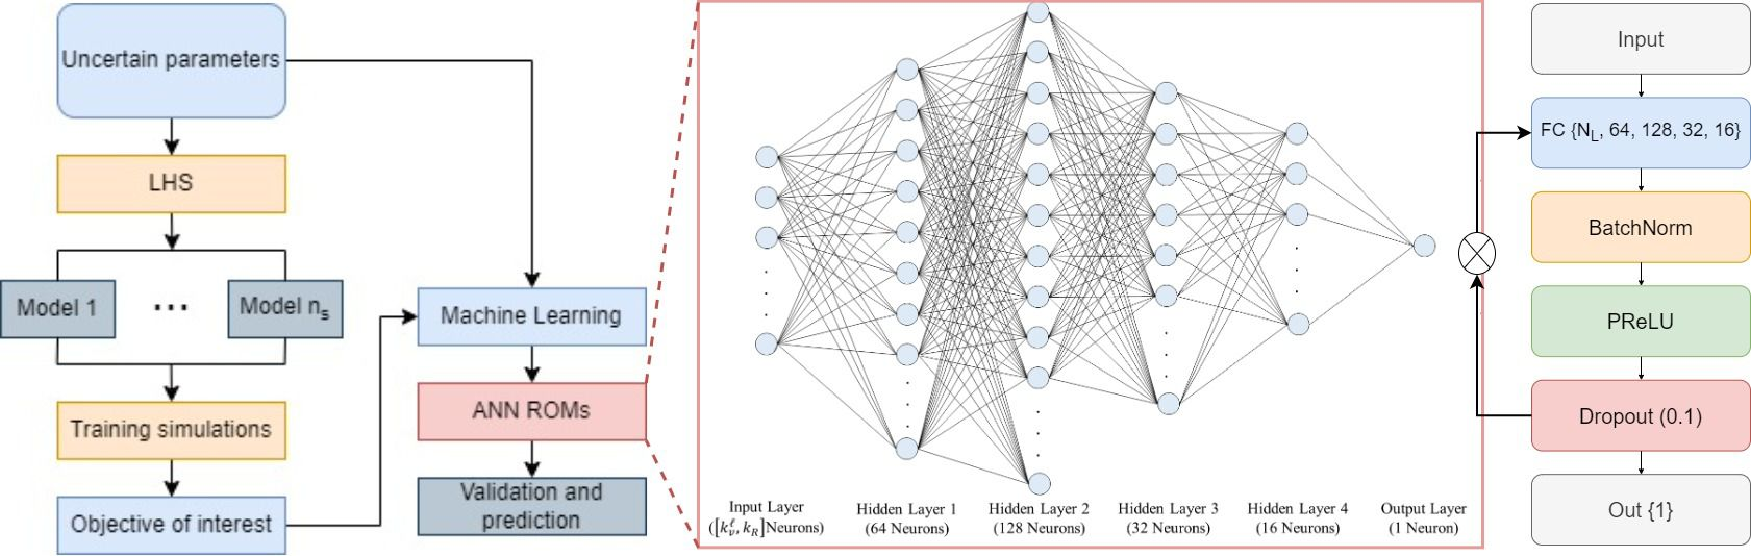
\includegraphics[width=16cm]{figs/Figure 1.pdf}
    \caption{Workflow diagram for machine learning-based ROM development.}
    \label{mlrom}
\end{figure}

\begin{enumerate}[Step 1.]
\item \textit{Experimental design}: Given a set of uncertain parameters $k_{v}^{\ell_d}$ and $k_R$, we generate $n_s$ training samples using Latin Hypercube Sampling (LHS) \citep{Iman2008, Helton2003LatinSystems}.
\item \textit{Forward simulations}: Physics-based HFS of CO$_2$ injection and post-injection migration is performed with each of the $n_s$ training samples using the Finite Element Heat and Mass Transfer (FEHM) simulator \citep{Zyvoloski1997}. 
\item \textit{Collect training data}: For each training realization, the set of uncertain parameters, monitoring data, and cumulative CO$_2$ leakage are collected. In Fig.\ref{mlrom}, we see that the uncertain parameters are inputs for the ROM training and the objectives of interest (cumulative CO$_2$ leakage and monitoring data) are the corresponding outputs. 
\item \textit{Train ROMs for the objectives of interest}: A reduced-order model is used to map the relationship between the training parameters inputs and outputs. We build an ensemble of ROMs, one for each objective of interest, namely the cumulative CO$_2$ leakage ($M_c$) and the simulated monitoring data ($D$) at each specified time-step. A fully-connected artificial neural network (ANN) is implemented to build the ROMs. Fig.\ref{mlrom} shows the architecture of the ANN.
\item \textit{Validate the ROMs against the HFS}: Using 10-fold cross-validation \citep{Xu2018249}, we test the predictions from the ROMs against the HFS results in order to perform hyper-parameter tuning and obtain robust ROMs that can be used for further predictions.
\end{enumerate}

Using the Python TensorFlow/Keras packages \citep{tensorflow2015-whitepaper, chollet2015keras}, we develop a fully-connected ANN architecture to build the ROMs. Each ANN consists of four hidden layers with sizes $64$, $128$, $32$, and $16$, respectively, with a total number of parameters equal to $14,705$. A kernel regularizer is applied with the $\ell_1$-norm, and dropout of $10\%$ is used on each hidden layer. The activation function is the parametric rectified linear unit (PReLU), which learns the negative slope for each batch in each epoch. The Adam optimizer \citep{Kingma2014Adam} is used with a mean squared error (MSE) loss function. Training is performed on an NVIDIA RTX A$6000$ GPU in about $2$ minutes for each ROM using $10$-fold cross-validation. The average validation MSE is approximately $8.5\times10^{-4}$ and the correlation coefficient ($R^2$) is approximately $0.98$. The truth vs. prediction performance for a set of $500$ realizations of uncertain parameters is shown in Fig.\ref{rom_train}.

\begin{figure}
    \centering
    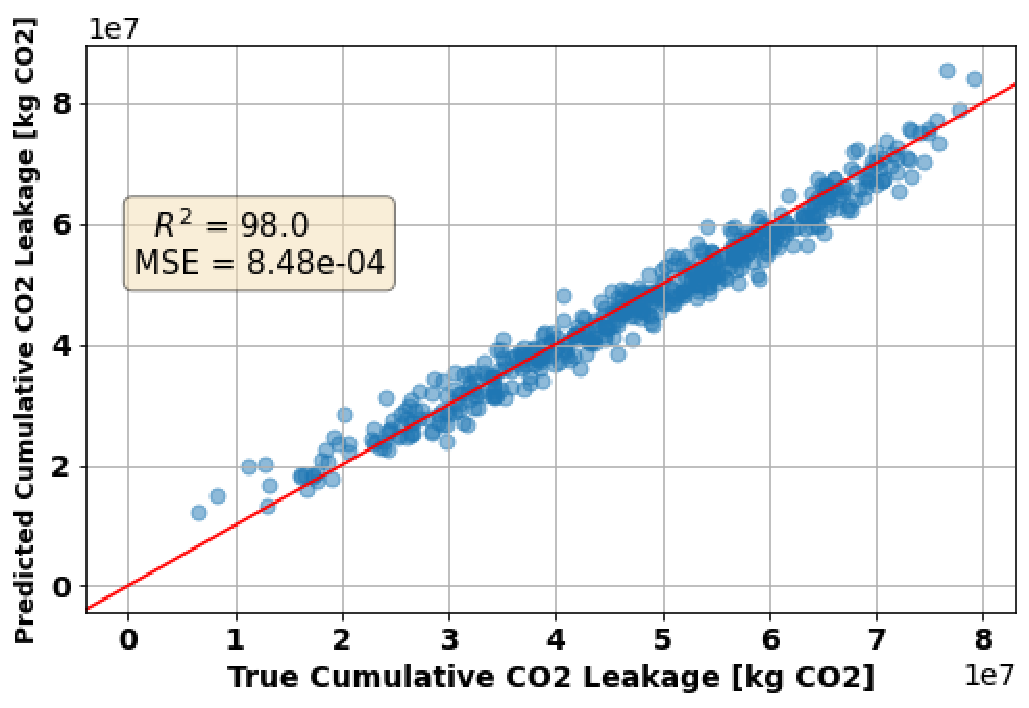
\includegraphics[width=8.5cm]{figs/Figure 3.pdf}
    \caption{Cumulative CO$_2$ leakage prediction from ANN ROM vs true cumulative CO$_2$ leakage.}
    \label{rom_train}
\end{figure}

\subsection{Workflow for Optimal Monitoring Design}
In this section we present a filtering and ROM based workflow for optimal monitoring design of GCS. The workflow diagram is shown in Fig. \ref{opt_workflow}. The main steps for the optimal monitoring design workflow are summarized below.

\begin{enumerate}[Step 1.]
\item \textit{Develop ROMs for the objective function, $M_c$, and predict monitoring data, $D$}: A detailed description of the ROM development workflow were presented in the previous section. We build one ROM for each monitoring data point, $d_i$, in each data vector $D^j$. The vector of predicted monitoring data is denoted as $O(m)=[O_1(m), O_2(m), \ldots,O_{n_d}(m)]^T$, where $m$ is the vector of uncertain model input parameters, namely $k_v^\ell$ and $k_R$. The ROMs are used to replace FEHM physics-based simulations and to predict the objectives of interest for a set of new input parameters not in the training data.

\item \textit{Generate an ensemble of realizations of monitoring data, $D$}: Initially, $l_d$ realizations are sampled from the prior PDF of $m$, and are denoted as $ \{\widetilde{m}^j\}_{j=1}^{\ell_d}$. The corresponding monitoring data, $\widetilde{d}_{obs}^j$, for each $\widetilde{m}^j$ are given by:
\begin{equation} \label{eq:4}
    \widetilde{d}_{obs}^j = O(\widetilde{m}^j) + e^j
\end{equation}
where $O(\widetilde{m}^j$ is the ROM prediction for $n_d$ monitoring data points and $e^j$ denotes the $j^{th}$ realization of measurement errors which follow a Gaussian distribution.

\item \textit{Generate Monte Carlo samples, and calculate prior uncertainty}: A large number ($50,000$) Monte Carlo samples are generated from the prior distribution of $m$, and denotes as $\{\hat{m}^k\}_{k=1}^{\ell_{MC}}$. The Monte Carlo samples are used to calculate the prior PDF and the amount of uncertainty in the prior can be computed using Eq. (\ref{eq:1}).

\item \textit{Filter the Monte Carlo samples, and compute expected posterior uncertainty}: Using a filtering-based method \citep{Caers2011}, also known as rejection sampling, we construct a posterior distribution of m conditional to each $\widetilde{d}_{obs}^j$. First, using the Monte Carlo samples, $\hat{m}^k$, generated in Step 3, we simulate the corresponding monitoring data $\hat{d}^k$ with the ROMs generated in Step 1, such that $\hat{d}^k=O(\hat{m}^k)$. Here, $\hat{d}^k$ represents a realization from the distribution of potential monitoring data sets that capture potential CO$_2$ leakage scenarios given the uncertain input parameters $k_v^\ell$ and $k_R$. The data assimilation error is defined as the maximum absolute error (MAE) as follows:
\begin{equation} \label{eq:5}
    MAE(d^j_{obs}) = \max\limits_{1\leq i \leq n_d} | \widetilde{d}^j_{obs,i} - \hat{d}^k_i | 
\end{equation}

Given a threshold value $\tau$, the $\hat{m}^k$ sample is accepted as a legitimate realization of the posterior distribution according to the following acceptance probability:
\begin{equation} \label{eq:6}
    P_{acc}(\hat{m}^k) = 
    \begin{cases}
      1, & \text{if}\ MAE<\tau \\
      0, & \text{otherwise}
    \end{cases}
\end{equation}

The threshold value, $\tau$, is chosen based on engineering judgement and takes into consideration the measurement and modeling errors. Therefore, $\hat{m}^k$ is accepted if it is deemed sufficiently consistent with the true monitoring data realization. Every Monte Carlo sample is evaluated using Eq. (\ref{eq:6}) and the accepted samples constitute the posterior distribution of m conditional to the monitoring data realization $\widetilde{d}^j_{obs}$ such that $\ell_d$ posterior samples of $m$ are obtained. The expected posterior uncertainty is calculated using Eq. (\ref{eq:2}). 

\item \textit{Calculate the expected amount of uncertainty reduction $U_R$}: The expected amount of uncertainty reduction, $U_R$, is calculated by comparing the uncertainty in the prior distribution and the expected value of the uncertainty in the posterior distribution using Eq. (\ref{eq:3}). 

\item \textit{Monitoring well placement optimization}: We repeat Steps 2-5 for every possible monitoring well location in the GCS area of review (AOR), conditional to the data for each possible measurement type, $D^j$. In order to accelerate the optimization procedure, we coarsen the simulation grid into a $4\times4$ subgrid, meaning there are $16$ possible monitoring well locations. We calculate the expected amount of uncertainty reduction for each monitoring data type, $D^j$, for each possible monitoring well location $\{{x^p}\}_{p=1}^{16}$, and obtain the monitoring design that maximally reduces the uncertainty in cumulative CO$_2$ leakage (maximally reducing the uncertainty is equivalent to minimizing the negative expected uncertainty reduction), as shown in Eq. (\ref{eq:7})
\begin{equation} \label{eq:7}
    x_p^* = \min\limits_{1\leq p \leq 16} -U_R^{x_p}
\end{equation}
This results in an exhaustive search in the subgrid to obtain the optimal well location, $x_p^*$, that yields the highest uncertainty reduction, defined by $U_R^{x_p}$ as follows:
\begin{equation} \label{eq:8}
    U_R^{x_p} = U^{x_p}[P(M_c)] - E_d[U^{x_p}[P(M_c \vert D^j]]
\end{equation}
\end{enumerate}

\begin{figure}
    \centering
    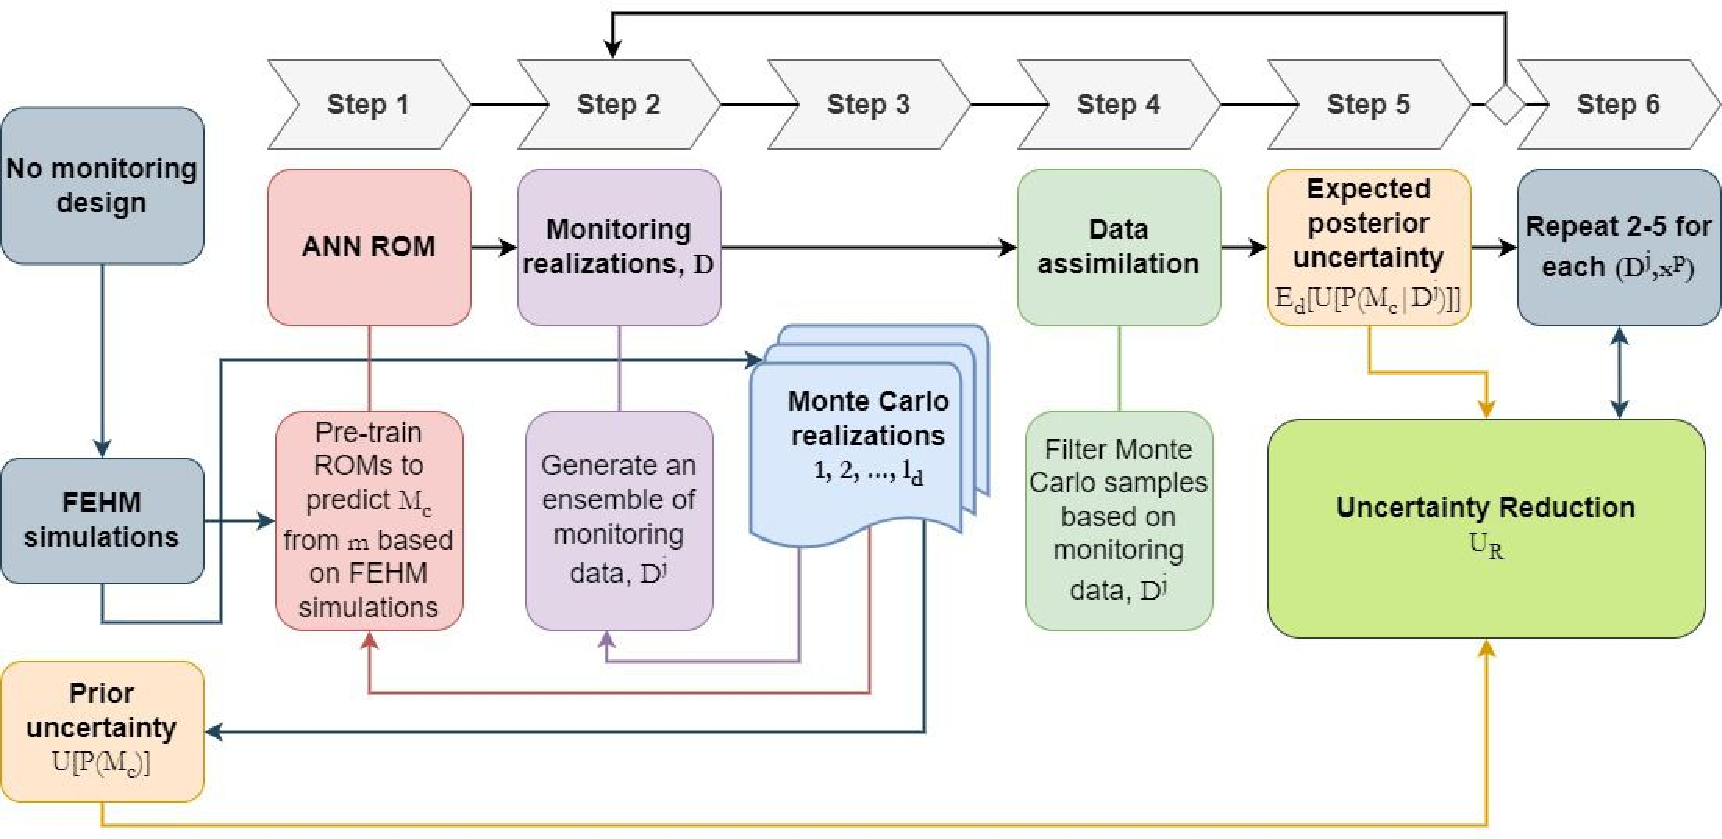
\includegraphics[width=16.5cm]{figs/Figure 4.pdf}
    \caption{Workflow diagram for optimal monitoring design. First, calculate the prior uncertainty with no monitoring design based on Monte Carlo samples of the FEHM simulations. Then use the pre-trained ROMs to predict CO$_2$ cumulative leakage using Monte Carlo samples and perform data assimilation of monitoring measurement $D^j$ for monitoring well placement $x^p$ to compute expected posterior uncertainty. The uncertainty reduction for case $(D^j,x^p)$ is given by $U^{x_p}[P(M_c)] - E_d[U^{x_p}[P(M_c \vert D^j]]$, and we repeat for each possible $D^j$ and $x^p$.}
    \label{opt_workflow}
\end{figure}

With this optimal monitoring design workflow, the expected uncertainty reduction in cumulative CO$_2$ leakage for each potential monitoring measurement and each potential monitoring well location can be computed, and the optimal monitoring design that reduces the uncertainty in the simulated amount of CO$_2$ leakage is obtained.

\subsection{Model Description}
We implement the optimal monitoring design workflow on a synthetic GCS model consisting of a heterogeneous storage reservoir, a homogeneous caprock layer and a homogeneous aquifer, as shown in the schematic of the base model in Fig. \ref{model}. The thickness of each of the three layers is $30$ $m$, and the model is $1$ $km$ wide in the horizontal dimensions. The depth from ground surface to the top of the model is $1000$ $m$. A CO$_2$ injection well is placed at the center of the reservoir and multiple potential leakage pathways traverse the caprock, where CO$_2$ could potentially leak into the aquifer. Note that only one possible leakage pathway is shown in Fig. \ref{model}, while we have considered several scenarios with multiple potential leakage pathways. The caprock and aquifer layers have a homogeneous permeability distribution equal to $1\times10^{-1}$ $m^2$ and $1\times10^{-13}$ $m^2$, respectively. The storage reservoir has a heterogeneous permeability distribution, as shown in Fig. \ref{perm_hete}. The base model is generated using a spherical variogram model \citep{Caers2005, Chen2017623} with major and minor correlation lengths of $680$ $m$ and $280$ $m$, respectively, with a major direction of $45^\circ$ from the positive $x$-axis.

\begin{figure}
    \centering
    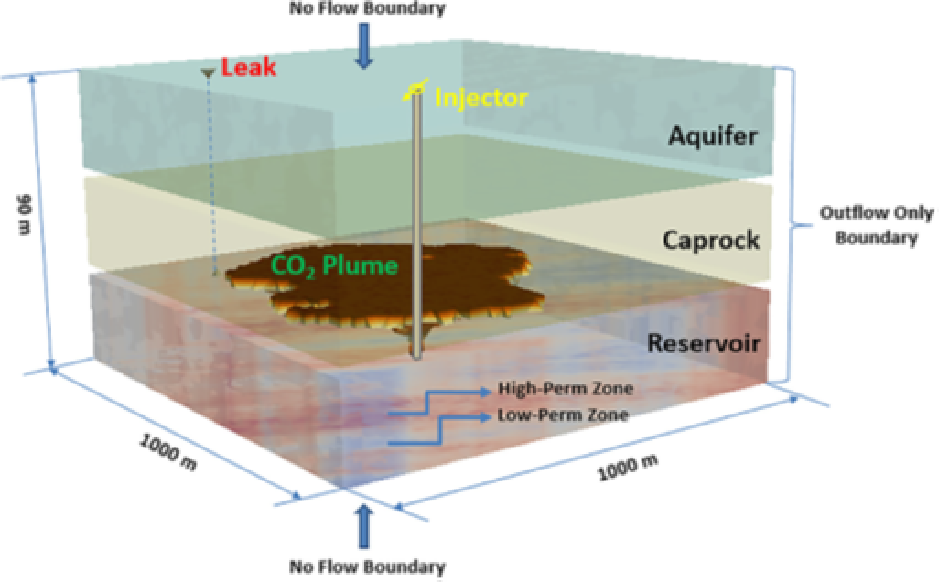
\includegraphics[width=10cm]{figs/Figure 5.pdf}
    \caption{Schematic of the base model, in which a storage reservoir and aquifer are separated by a caprock. At the center is a CO$_2$ injection well. The vertical axis is exaggerated 7 times.}
    \label{model}
\end{figure}

The mean of the permeability field is $1\times10^{-13}$ $m^2$. For each realization, we assume that the reservoir permeability is uncertain, and to honor this uncertainty we use a permeability multiplier, $k_R$, to multiply the aforementioned base permeability distribution. The lower and upper bounds for the multiplier $k_R$ and the potential leaky pathways $k_v^\ell$ are shown in Table \ref{tbl:1}. 

\begin{figure}
    \centering
    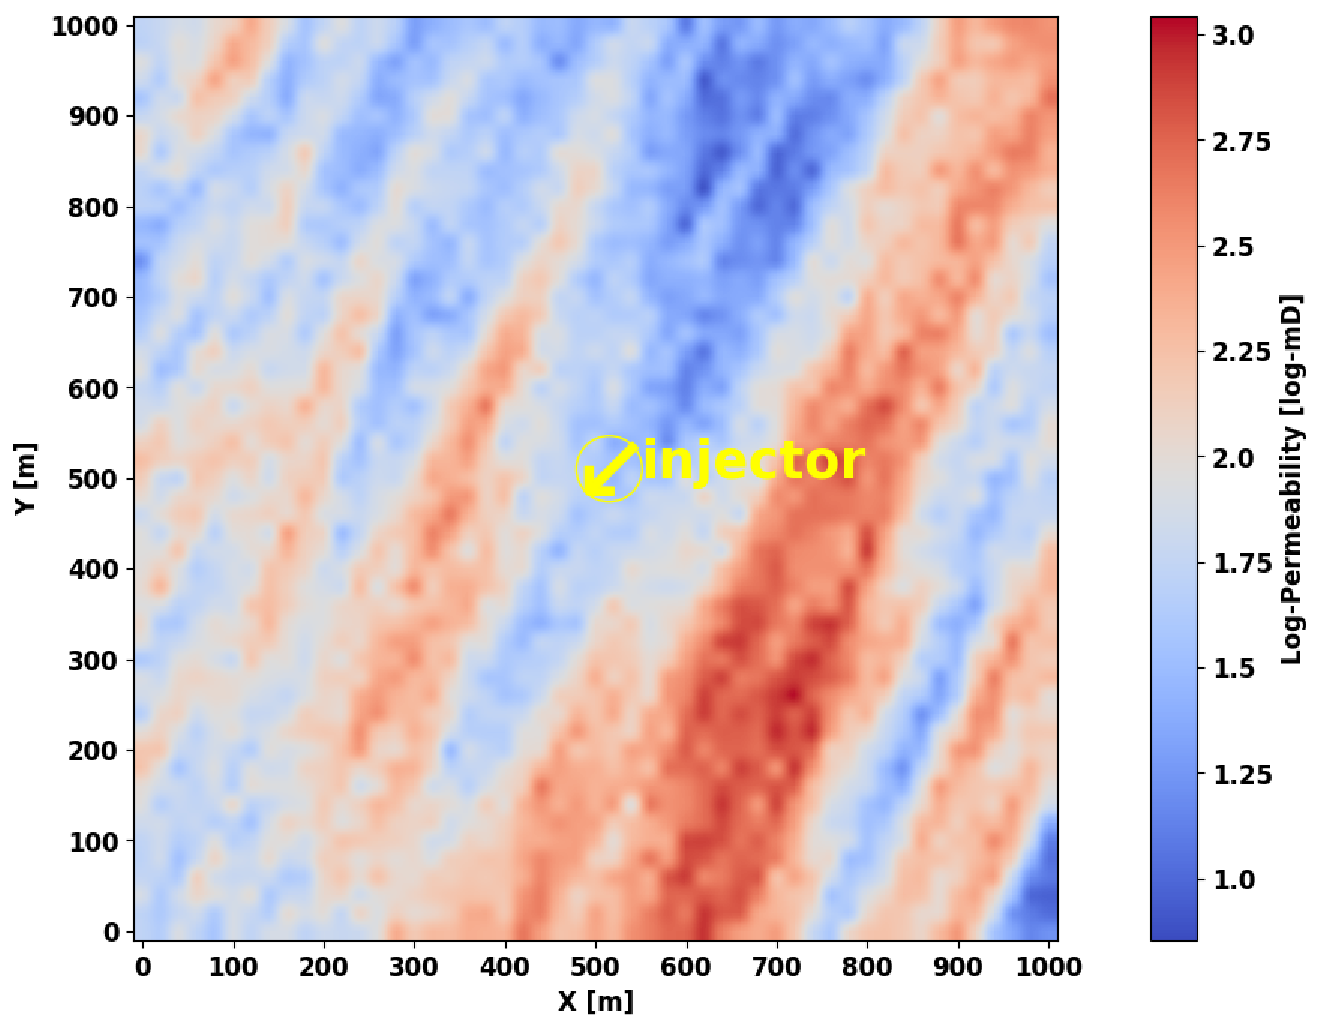
\includegraphics[width=10cm]{figs/Figure 6.pdf}
    \caption{Log-permeability distribution of the base model. The darkest blue color corresponds to the lowest permeability, while the darkest red color corresponds to the highest. The yellow circle with an arrow indicates the CO$_2$ injection well.}
    \label{perm_hete}
\end{figure}

\begin{table}[width=.9\linewidth,cols=5,pos=h]
    \caption{Uncertain parameters and their lower and upper bounds.}\label{tbl:1}
    \begin{tabular*}{\tblwidth}{@{} LLLLL@{} }
    \toprule
    \textbf{Uncertain parameters} & \textbf{Symbol} & \textbf{Lower bound} & \textbf{Upper bound} & \textbf{Unit} \\
    \midrule
    Reservoir permeability multiplier & $k_R$ & 0.5 & 2 & $-$ \\
    \multirow{2}{*}{Permeability of leaky pathway(s)} & \multirow{2}{*}{$k_v^\ell$} & -19 & -14 & $log_{10}$ $[m^2]$ \\ &  &  0.001 & 10 & $mD$ \\ 
    \bottomrule
    \end{tabular*}
\end{table}

A numerical mesh for the reservoir simulation is made using the grid generation toolkit \textit{LaGriT} \citep{George1999}. The numerical mesh has 51 grid nodes in both the $x$- and $y$-directions, and 31 grid nodes in the $z$-direction. The distance between each grid node in the x- and y-directions is 20 $m$, and in the $z$-direction it is 3 m. The total number of grid nodes used in the simulation is 80,631, with 26,010 grid nodes in the reservoir and caprock, respectively, and 28,611 grid nodes in the aquifer. FEHM is used for 3D multi-phase flow simulations \citep{Zyvoloski1997}. The boundary conditions of the reservoir are defined as Dirichlet boundaries, allowing CO$_2$ to flow out but not in, and water pressure above hydrostatic. The top and bottom boundary conditions of the simulation model are no-flow boundaries. The thermal conditions of the model are initialized using a geothermal gradient of $0.03^\circ$C/m with a temperature of $20^\circ$C at the top. Pressure gradients are initialized at $9.81\times10^{-3}$  MPa/m with a pressure of 0.2 MPa along the top. In this study, CO$_2$ is constantly injected in a five-year period, monitored monthly, with a constant injection rate of 0.1 million metric tons/year.

%%%%%%%%%%%%%%%%%%%%%%%%%%%%%%%%%%%% Results
\section{Results}
In this section we apply our optimal monitoring design workflow using the ANN ROMs and filter-based uncertainty quantification approach to obtain the optimal monitoring well placement and monitoring measurement data type for two synthetic GCS examples.

\subsection{Workflow Validation}
We validate the workflow for optimal GCS monitoring design using a simple example. Fig. \ref{perm_hete} shows the log-permeability distribution for the base model with a CO$_2$ injection well at the center, noted with a yellow circle and arrow. All the monitoring data in this study are collected in the aquifer zone, similar to monitoring at the above zone monitoring interval (AZMI) in the work of \citet{Sun2013}. The monitoring frequency is once per month for the duration of 5 years injection, resulting in 60 monitoring data points. The objective function, $M_c$, is the cumulative CO$_2$ leakage at the end of 5 years. In the model, we set up three material zones corresponding to the three adjacent formations, namely the storage reservoir, caprock, and aquifer. The cumulative CO$_2$ saturation in each zone can be output from the FEHM simulation results, and the cumulative leakage is computed by summing the CO$_2$ mass in the aquifer and caprock layers. Our approach for monitoring design involves quantifying the uncertainty reduction by monitoring pressure, CO$_2$ saturation, or temperature at each potential monitoring well location. 

The data assimilation error tolerance, $\tau$ from Eq. (\ref{eq:6}), for pressure is set equal to 0.002 MPa, while for CO$_2$ saturation it is 0.05, and for temperature it is 0.002$^\circ$C. Note that the choice of $\tau$ is site and case specific and is based on engineering judgement that takes into consideration the measurement and modeling error.

Two case studies are considered in this study: (1) GCS project with 3 potential leakage pathways, and (2) GCS project with 6 potential leakage pathways. The uncertain parameters are the permeability multiplier, $k_R$ for the storage reservoir, and the $\ell$ permeability values for the $\ell$ potential leakage pathways, where $\ell=3$ and $\ell=6$, respectively. The total number of uncertain parameters, $u^\ell$ are 4 and 7, respectively. The lower and upper bounds for the uncertain parameters are shown in Table \ref{tbl:1}. For each case study, we run 500 training simulations generated by LHS with $u^\ell$ uncertain parameters. Each HFS requires approximately 22 minutes. We perform parallelization on an 8-node cluster, and the total simulation time is approximately 23 hours to finish all 500 training realizations. Fig. \ref{cases} shows the base model for Case 1 and Case 2 respectively.

\begin{figure}
    \centering
    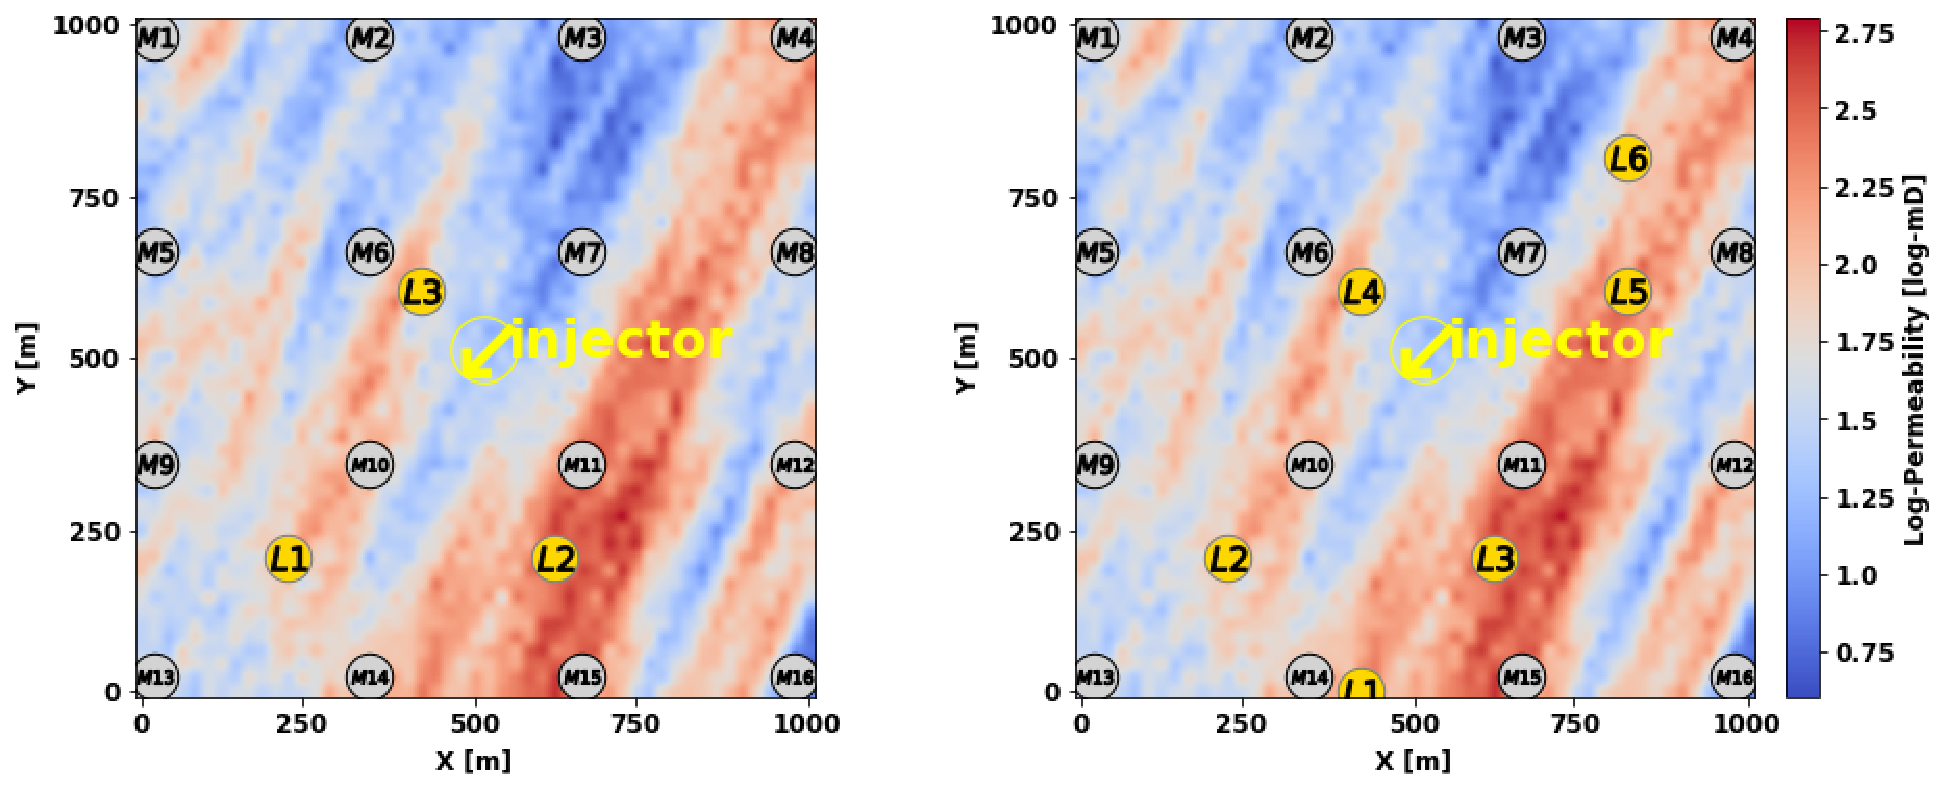
\includegraphics[width=15cm]{figs/Figure 7.pdf}
    \caption{Log-permeability distribution of the base model for Case 1 (left) with 3 potential leaky pathways, and Case 2 (right) with 6 potential leaky pathways. The dark yellow circles labeled $L_i$ represent the leakage pathways, light gray circles labels $M_i$ are the possible monitoring well locations, and the yellow circle with an arrow is the CO$_2$ injection well.}
    \label{cases}
\end{figure}

We choose one simulation from the 500 training realizations in Case 1 to show when CO$_2$ leakage occurs. The values of the different parameters for the chosen model are shown in Table \ref{tbl:2}. The cumulative CO$_2$ leakage over the GCS project time is shown in Fig. \ref{cum_leak_line}. Figure \ref{cum_leak_map} shows the leaked CO$_2$ saturation distribution at the top of the aquifer. It can be seen that CO$_2$ leakage occurs after about 210 days of injection. We observe that CO$_2$ is leaking through the potential pathway $L_3$, which is 141.4 $m$ away from the injector, while no leakage occurs at potential pathways $L_1$ and $L_2$ after 5 years of injection. For this specific example, it is important to note that the permeability of $L_3$, $k_v^3$ is higher than that of $L_1$ and $L_2$.

\begin{table}[width=.9\linewidth,cols=3,pos=h]
    \caption{The parameters for one chosen model from the 500 training realizations in Case 1.}\label{tbl:2}
    \begin{tabular*}{\tblwidth}{@{} LLL@{} }
    \toprule
    \textbf{Parameters} & \textbf{Value} & \textbf{Unit}  \\
    \midrule
    CO$_2$ injection rate & 3.17 & kg/s \\
    Thickness of caprock layer & 30 & m \\
    Permeability of 1$^st$ potential leakage pathway & $2.19\times 10^-{17}$ & $m^2$ \\
    Permeability of 2$^nd$ potential leakage pathway & $3.37\times 10^-{17}$ & $m^2$ \\
    Permeability of 3$^rd$ potential leakage pathway & $2.97\times 10^-{16}$ & $m^2$ \\
    Distance between injector and 1$^st$ potential leakage pathway & 424.3 & m \\
    Distance between injector and 2$^nd$ potential leakage pathway & 360.6 & m \\
    Distance between injector and 3$^rd$ potential leakage pathway & 141.4 & m \\
    Permeability for aquifer layer & $1\times 10^{-13}$ & $m^2$ \\
    Permeability for caprock layer & $1\times 10^{-19}$ & $m^2$  \\
    Reservoir permeability multiplier & 1.88 & $-$   \\  
    \bottomrule
    \end{tabular*}
\end{table}

\begin{figure}
    \centering
    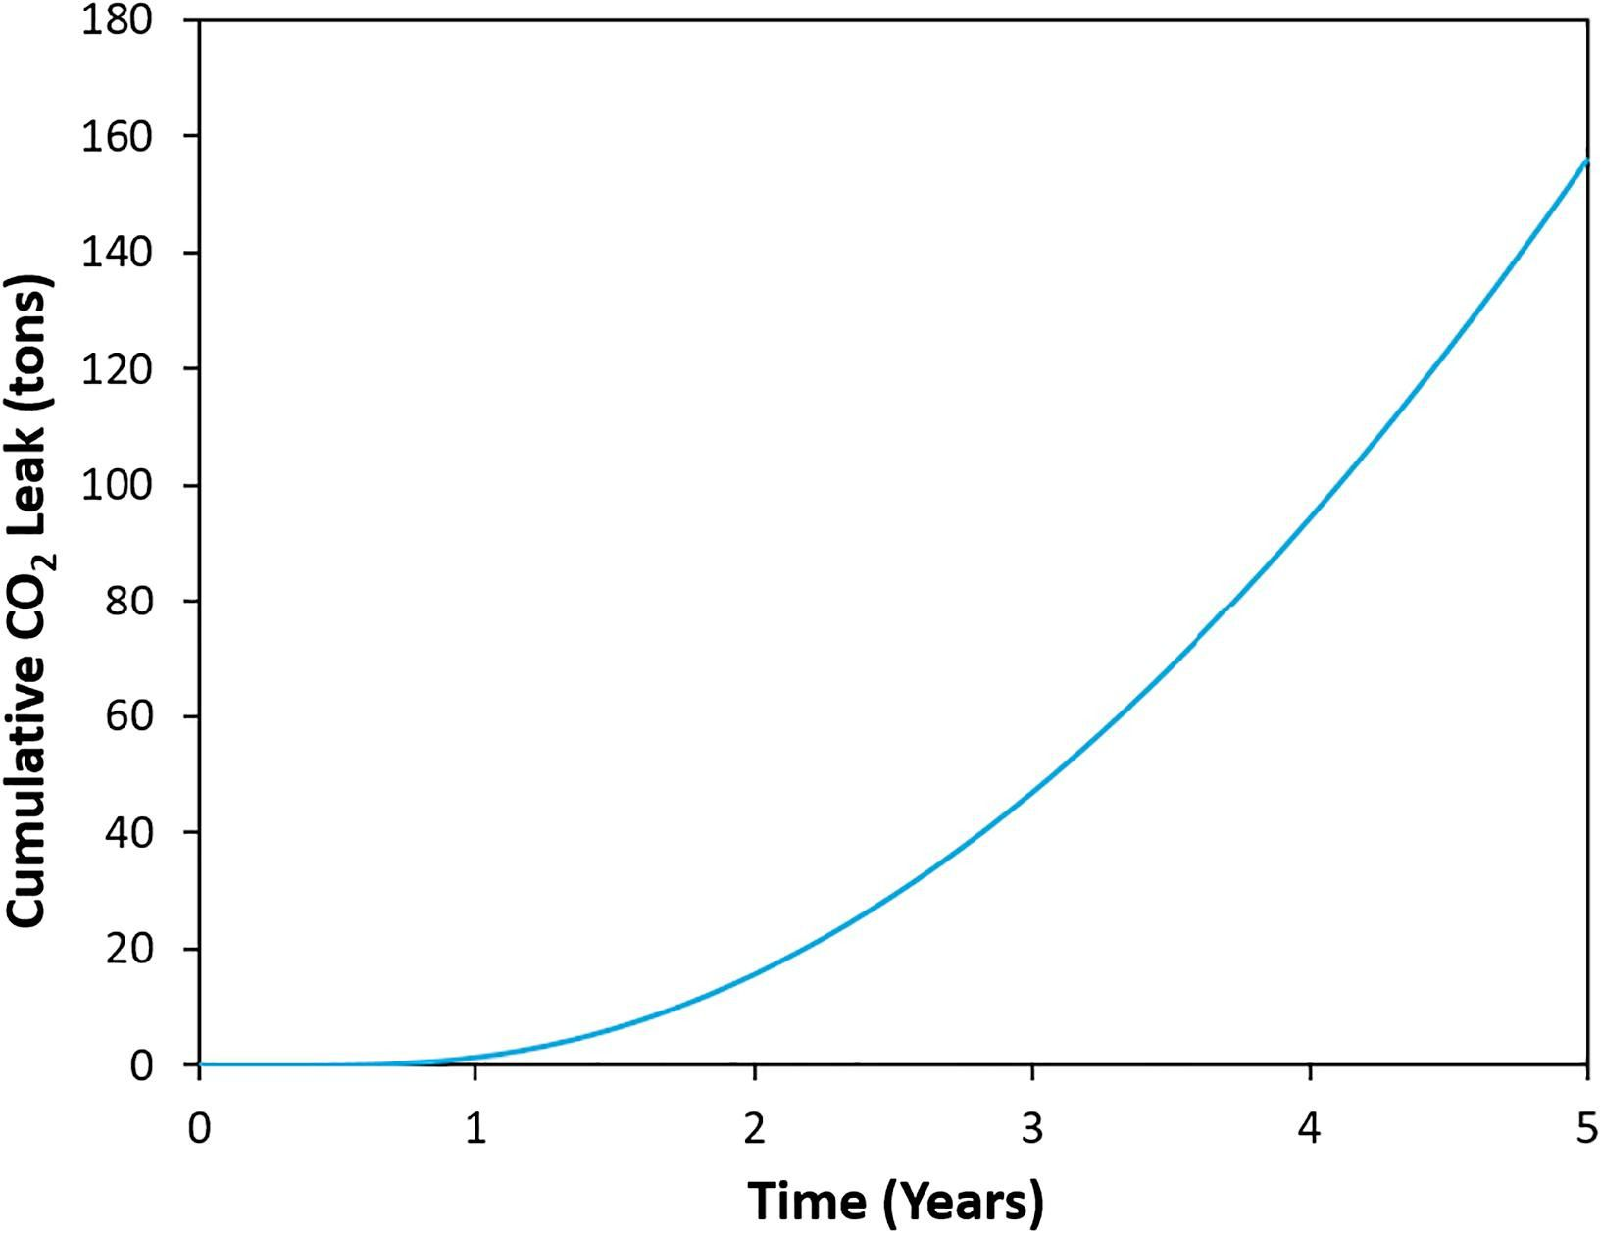
\includegraphics[width=7.5cm]{figs/Figure 8.pdf}
    \caption{Cumulative CO$_2$ leakage over time computed for one chosen training realization in Case 1.}
    \label{cum_leak_line}
\end{figure}

\begin{figure}
    \centering
    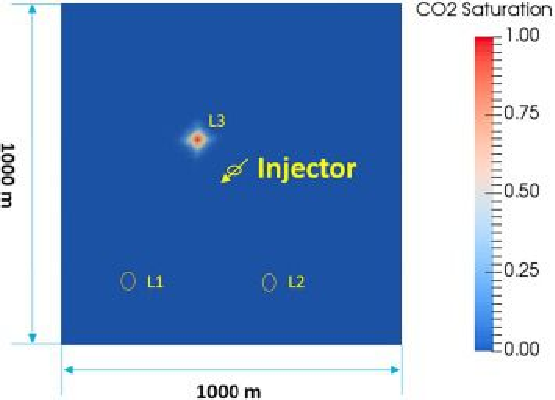
\includegraphics[width=8.5cm]{figs/Figure 9.pdf}
    \caption{Plan view (top of the aquifer) of CO$_2$ leakage at the end of 5 years of injection based on one chosen training realization in Case 1. Yellow circles indicate the potential leakage pathways. Units for CO$_2$ saturation is fraction.}
    \label{cum_leak_map}
\end{figure}

For each case, the 500 training realizations are used to train ROMs for the monitoring data and cumulative CO$_2$ leakage using the ANN architecture in Fig \ref{mlrom}. Fig. \ref{rom_train} shows the quality of the ROMs tested by 10-fold cross-validation \citep{Geisser1993, Xu2018249}. The MSE and $R^2$ are $8.5\times10^{-4}$ and $0.98$, respectively. This proves that the fidelity of ROMs to the numerical simulations is high at the advantage of a much lower computational cost.

With the proposed workflow, the expected uncertainty reduction of the cumulative CO$_2$ leakage can be computed for each of the 16 possible monitoring well locations, for each monitoring measurement type. For each data set, 200 possible realizations of monitoring data are generated following Step 2 in Section 2.4. To obtain the expected uncertainty reduction using Eq. (\ref{eq:3}), the prior uncertainty $U[P(M_c)]$ and posterior uncertainty $U[P(M_c \vert D^j)]$ corresponding to each possible monitoring data realization $D^j$ for each possible well location $x^p$ should be computed. Higher uncertainty reduction of the objective function indicates greater VOI in the monitoring data obtained from the optimal well location and monitoring measurement type. Through these examples, we can see that our proposed workflow can be effectively used to determine optimal CO$_2$ monitoring design from a set of alternative monitoring designs.

We observe that monitoring for pressure provides the highest uncertainty reduction in general, followed by CO$_2$ saturation and lastly pressure. The spatial distribution of uncertainty reduction in CO$_2$ leakage is shown in Fig. \ref{heatmaps} for every possible well location $x^p$ in the $4 \times 4$ subgrid, and point-wise comparison of the uncertainty reduction at each monitoring well location for each measurement type is shown in Fig. \ref{point_ur}. One can observe that placing a monitoring well at location 6 and assimilation the pressure measurements provides the highest uncertainty reduction possible in the monitoring design for both Case 1 and Case 2. For Case 1, the optimal monitoring design given by $(pressure, x^6)$ yields an uncertainty reduction in the cumulative leakage of CO$_2$ of approximately 29.42$\times 10^3$ metric tons (29.24 kt), while the optimal design for CO$_2$ saturation and temperature monitoring yield an uncertainty reduction of approximately 19.34 kt and 17.71 kt, respectively. Similarly, for Case 1, the optimal monitoring design given by $(pressure, x^6)$ yields an uncertainty reduction of 26.29 kt of cumulative CO$_2$ leakage, while the optimal design for CO$_2$ saturation and temperature monitoring yield an uncertainty reduction of approximately 16.94 kt and 16.29 kt, respectively.

\begin{figure}
    \centering
    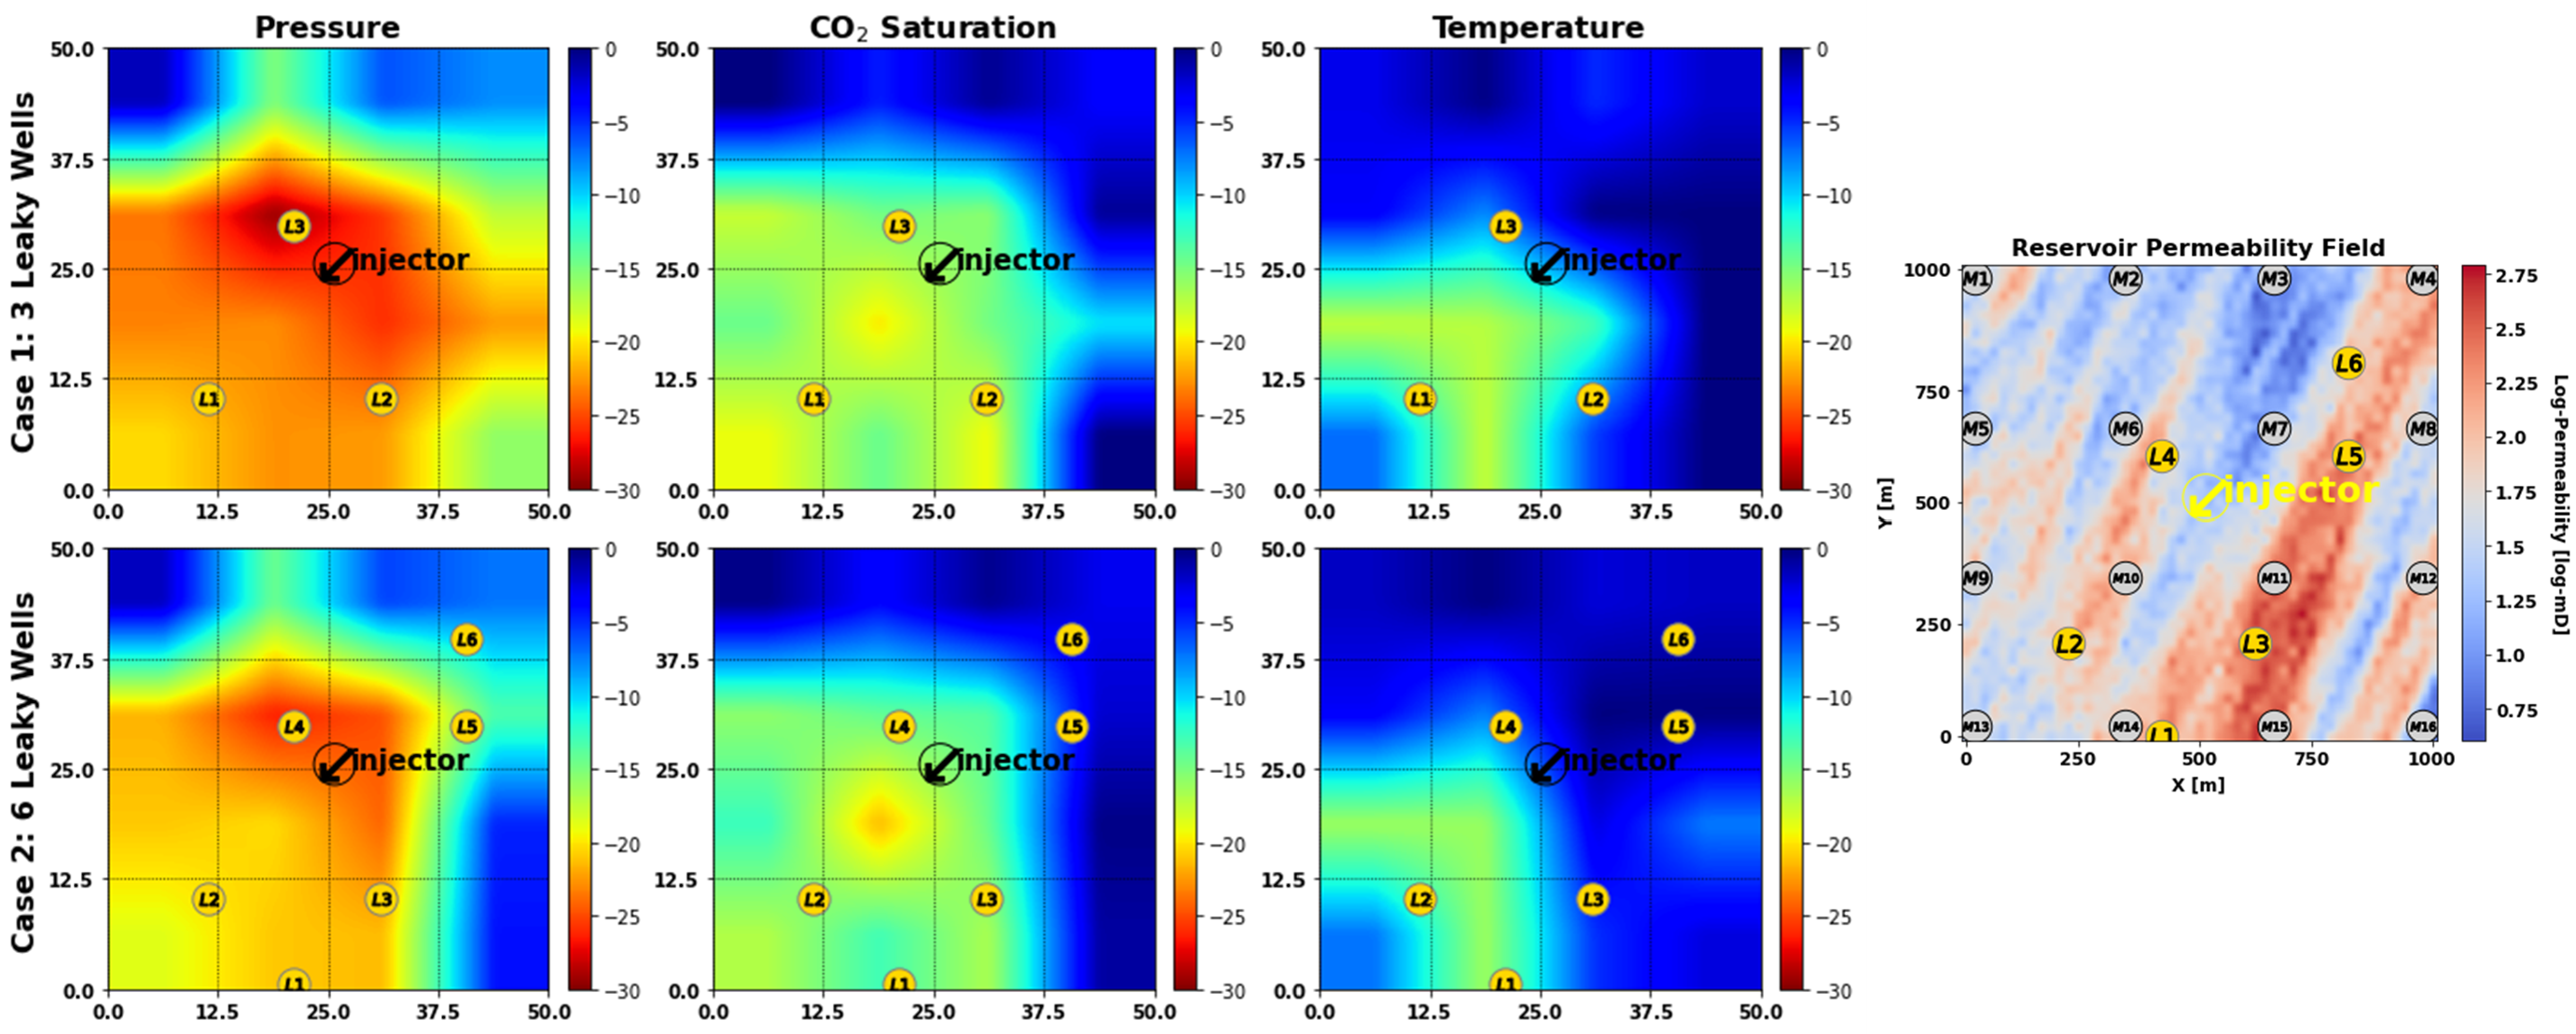
\includegraphics[width=16.5cm]{figs/Figure 10.pdf}
    \caption{Left: Plan view (top of the aquifer) of the uncertainty reduction obtained by all possible monitoring well locations. Top row represents Case 1 with 3 leakage pathways, and the bottom row represents Case 2 with 6 leakage pathways. Each column represents monitoring data for pressure, CO$_2$ saturation, and temperature, respectively. Right: Plan view of the reservoir permeability field with possible leakage pathways (yellow) and all possible monitoring well locations (gray).}
    \label{heatmaps}
\end{figure}

\begin{figure}
    \centering
    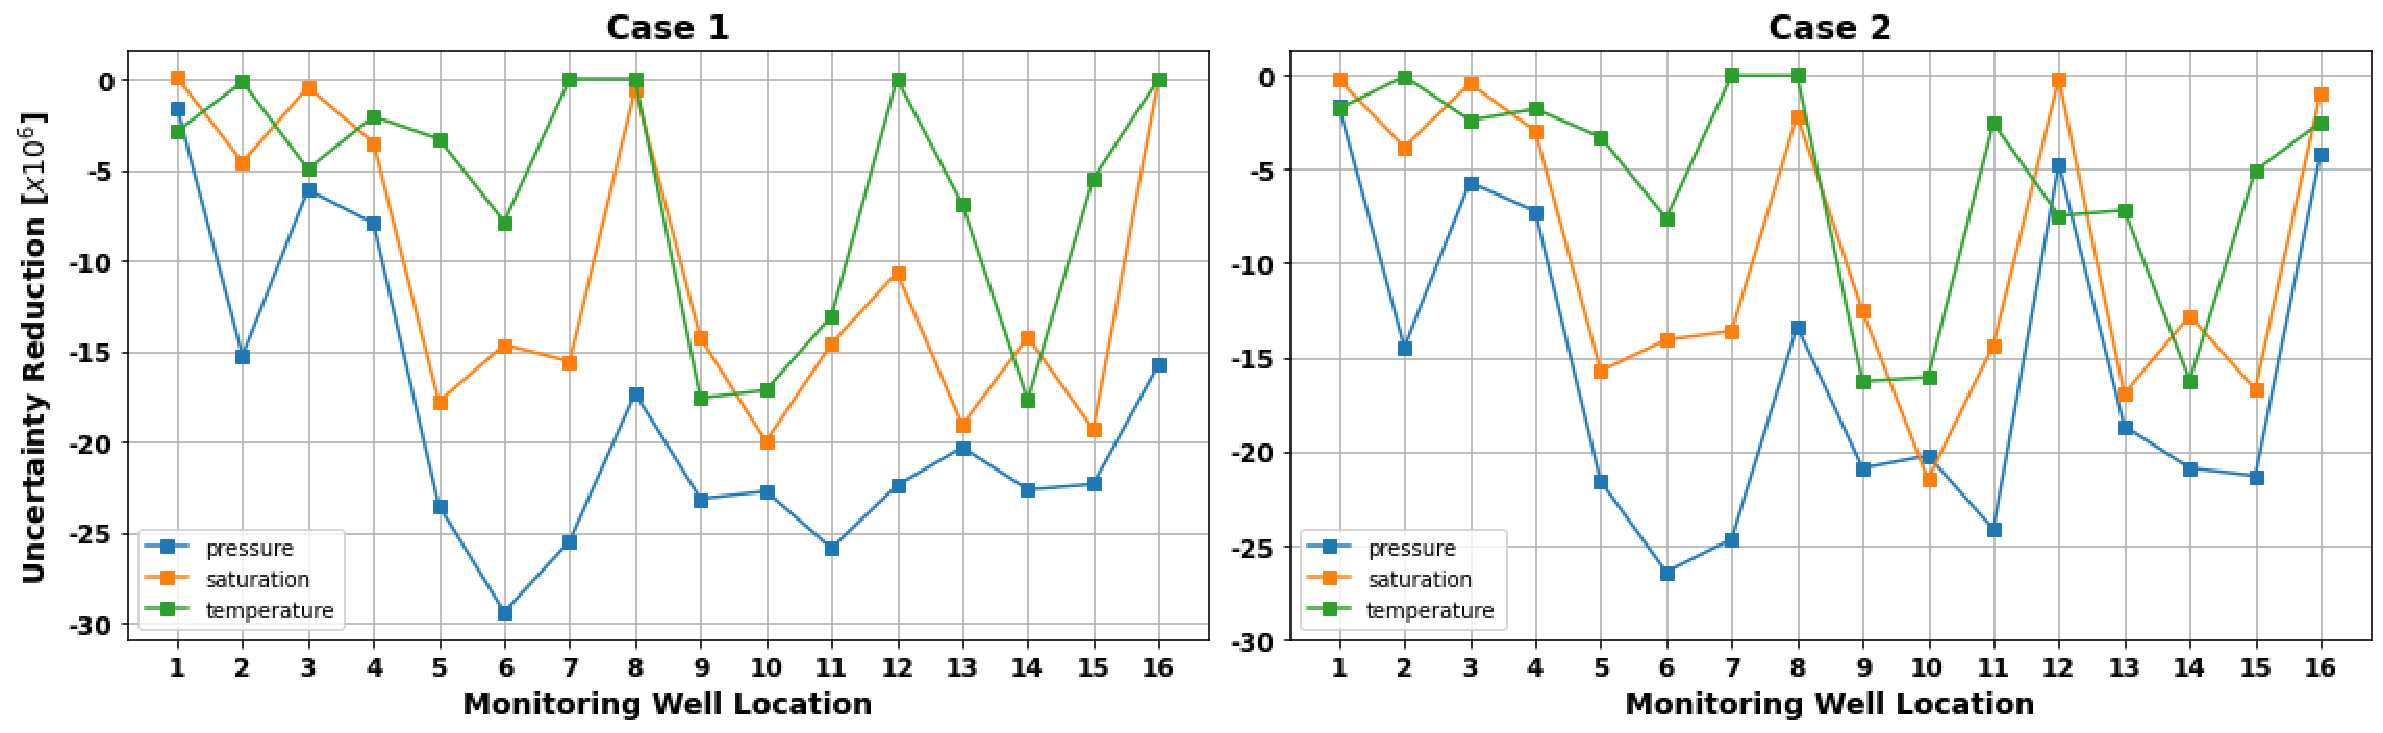
\includegraphics[width=16cm]{figs/Figure 11.pdf}
    \caption{The point-wise calculated uncertainty reduction at each possible monitoring well location for each measurement type. Case 1 is shown on the left, and Case 2 on the right.}
    \label{point_ur}
\end{figure}

The histograms for the prior and posterior distributions of the objective function obtained from the data realizations 1 and 100 for Case 1 and 2, respectively, are show in Fig. \ref{ur_dist}. The prior distribution is generated using LHS from the set of uncertain input parameters, $k_V^\ell$ and $k_R$, with a uniform distribution and calculating the cumulative CO$_2$ leakage using the ROMs. The posterior distribution for two random realizations, namely realization 1 and 100, are shown. These two are selected given that they had a relatively high amount of cumulative CO$_2$ leakage. Recall that the total uncertainty reduction, $U_R$ is given by the difference between the expected posterior uncertainty (the expected value of the ensemble of realizations) and the prior uncertainty distribution. The variances of the posterior distributions calculated show significant reduction in uncertainty of cumulative CO$_2$ leakage compared to the priors. The optimal monitoring design $(pressure, x^6)$ yields a reduction in cumulative CO$_2$ leakage uncertainty of approximately 29.24 kt. 

\begin{figure}
    \centering
    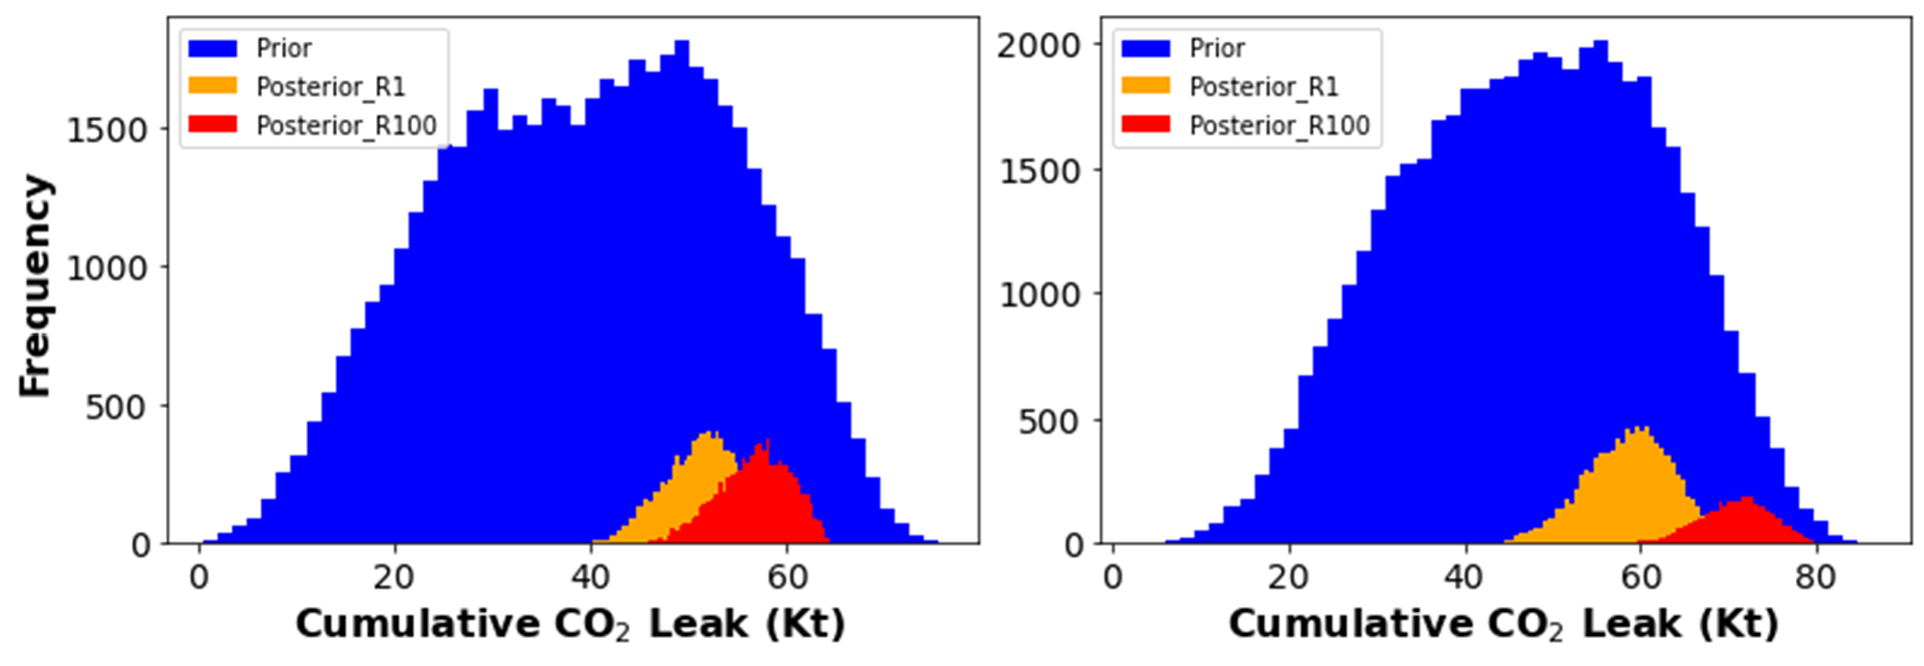
\includegraphics[width=16cm]{figs/Figure 12.pdf}
    \caption{The histograms for the prior (blue) and posterior distributions obtained at the optimal monitoring design from the data realizations 1 (orange) and 100 (red) for Case 1 (left) and Case 2 (right), respectively.}
    \label{ur_dist}
\end{figure}

\subsection{Discussion}
GCS monitoring operations require detailed data processing and interpretation in order to accurately quantify and potentially minimize leakage risks. Associated costs of performing monitoring operations requires evaluating the potential value of monitoring measurement type, and optimal monitoring well location, before the actual monitoring strategy takes place in the field. The workflow proposed can be used to select an optimal monitoring design that is robust under multiple potential leakage scenarios. Previous efforts in characterizing the geologic uncertainty in GCS projects show the importance and effect of these parameters \citep{Jia2018104, Chen2020, Pawar2022}, selecting the optimal measurement type \citep{Yonkofski2016, Oladyshkin2013671}, or selecting the optimal monitoring well location \citep{Sun2013, Sun2019}. Our work provides a framework to unify these three concepts under a single optimal monitoring design framework.

The slight difference in uncertainty reduction between Case 1 and Case 2, despite the fact that we have more leakage pathways, can be attributed to the fact that the main source of uncertainty is the geologic parameters, namely $k_v^\ell$ and $k_R$, rather than the number of leakage pathways. These parameters ultimately control the leaking of CO$_2$, and can range between very small ($\sim 0.001 mD$) to medium ($\sim 10 mD$). Thus, the cumulative CO$_2$ leakage does not directly correlate with having more or less leakage pathways, but with the permeability of the leakage pathways, $k_V^\ell$, and the reservoir permeability multiplier, $k_R$. For instance, wells 6-7 and 10-11 lie closest to the injection well at approximately 176.8 $m$, yet well 6 yields the highest uncertainty reduction since it is closest to a high permeability streak, similar to well 11. On the other hand, wells 7 and 10 lie on low permeability streaks, making the plumes travel relatively slower. Therefore, distance from injector and leakage pathways is important, but mostly controlled by the permeability heterogeneity in the reservoir.

Furthermore, it is evident that monitoring for pressure data yields the highest uncertainty reduction out of the three possible measurement types. This is due to the fact that the pressure plumes travel the fastest along a given subsurface formation, followed by saturation plumes and temperature plumes, in that order \citep{Chadwick2006303}. Temperature plumes tend to travel the least, given the thermal equilibrium of deep underground formations and the gradual enthalpy change in the reaction of CO$_2$ in saline aquifers \citep{koschel2006enthalpy}. In some monitoring locations, such as wells 7 and 8, monitoring for temperature provides little to no uncertainty reduction whatsoever, while pressure monitoring yields about 17-25 kt reduction. The total uncertainty reduction given by the sum of all three measurements correlated primarily with the pressure monitoring data, and assimilating multiple measurements types simultaneously does not necessarily add linearly, and tends to be dominated by a single measurement. Refer to \citet{Chen2018} for more information on assimilating multiple measurement types simultaneously.

It is also important to note that the monitoring wells are only drilled through the aquifer, and not the caprock and reservoir, thus only collecting monitoring measurements at the aquifer zone. This is way, despite $x^6$ being further away from the injector than the closest leakage pathway ($L_3$ in Case 1 and $L_4$ in Case 2), it still provides the most information about CO$_2$ leakage into the aquifer zone. Also, recall the aquifer is geologically homogeneous, and the pressure, CO$_2$ saturation, and temperature response does not necessarily exactly correlate with the reservoir response.

Regarding the monitoring well location grid, location $x^6$ yields the highest uncertainty reduction when using pressure measurements for both Case 1 and Case 2. However, the 16 possible monitoring well locations exist on a coarse $4\times 4$ subgrid. Monitoring location $x^6$ is closest to the injection well and a leakage pathway in both Case 1 and Case 2, and therefore provides the best uncertainty reduction. However, if a finer monitoring well location grid were used, say $16 \times 16$ or $32 \times 32$ (which is still coarser than the simulation grid at $51 \times 51$), a location between the injector well and $L_3$ in Case 1 and $L_4$ in Case 2 would most likely yield the best uncertainty reduction. This is due to the fact that a monitoring well in that location would be able to detect the CO$_2$ plume before it even reaches and leakage pathways, and would still be in the region of high permeability in the reservoir, thus yielding the best uncertainty reduction in cumulative CO$_2$ leakage. 

Moreover, given that we are using a coarse monitoring well location grid, several locations such as $M_{1-4}$, $M_8$, $M_{12}$, and $M_{14-15}$ yield little to no uncertainty reduction. We stipulate that this occurs because the CO$_2$ plume reaches the leakage pathways before it reaches these monitoring wells, and therefore provide little information to the data assimilation to reduce the uncertainty in leakage. This also leads to the idea that most of the CO$_2$ leakage is occurring in the pathways closest to the injection well, and thus the closer monitoring locations provide a better uncertainty reduction than those in the boundaries or further away. This relates to the fact that despite Case 2 having more leakage pathways, the uncertainty reduction in kt of CO$_2$ is not much different from that of Case 1.

Even though the examples used in our study to demonstrate how monitoring data from a shallow aquifer can be used, the proposed workflow can be extended and applied to monitoring data collected at any location and time within the GCS project. The potential value of such monitoring data can be evaluated by the presented workflow. Furthermore, placing several monitoring wells can provide a slight advantage compared to a single injector-monitor pair, but is impractical in field applications. Moreover, using several monitoring measurement types simultaneously provides little to no advantage compared to pressure monitoring. Refer to \citet{Chen2018} for further details.

At a CO$_2$ storage field operation, an optimal monitoring schedule and location based on the VOI described in this work can be used to collect the best possible monitoring data. The monitoring data can be assimilated to calibrate the uncertain model parameters using traditional data assimilation methods such as EnKF \citep{Evensen20091} or ES-MDA \citep{Emerick20133}. The calibrated models can be used to improve the accuracy in prediction for future and long-term behavior of the injected CO$_2$.

%%%%%%%%%%%%%%%%%%%%%%%%%%%%%%%%%%%% Conclusions
\section{Conclusions}
In this study, a workflow based on a machine learning reduced-order modeling technique and uncertainty quantification method within an optimization loop is proposed for geologic CO$_2$ sequestration monitoring design. We use the uncertainty reduction in cumulative CO$_2$ leakage as the quantity of interest to measure the potential value of monitoring measurement data. The optimal monitoring design yields an uncertainty reduction of approximately 29.94 kt in CO$_2$ leakage. The following conclusions have been drawn from this research:
\begin{enumerate}
    \item The proposed workflow can generate reasonable values of uncertainty reduction in different risk metrics at CO$_2$ storage site, including cumulative CO$_2$ leakage by utilizing different monitoring designs and has been demonstrated using a synthetic GCS project. The optimal monitoring design is obtained my assimilating pressure data at monitoring well location 6.
    
    \item The effect of different types of measurements (pressure, CO$_2$ saturation, and temperature) and the effect of monitoring well location on the choice of monitoring design is investigated. It is observed that pressure data has more value of information compared to CO$_2$ saturation, while temperature has the least value of information, though still valuable in terms of uncertainty reduction compared to no monitoring strategy.
    
    \item Well placement optimization is important to maximize the value of information for the monitoring design. Typical operations include pairs of one monitoring well for each injection well, partly due to the cost of drilling and data acquisition. Determination of the best location provides significant benefits in reducing the uncertainty of cumulative CO$_2$ leakage and ensure an efficient risk management in the life-cycle of a GCS project.
    
    \item The incremental reduction in uncertainty in the cumulative CO$_2$ leakage may not increase proportional to the distance from the injection well, and is a strong function of the reservoir permeability heterogeneity. Thus, an optimal monitoring well placement and measurement type is important to minimize present and future potential risks.
    
    \item The subgrid for the possible monitoring well locations will have a major impact in the optimal monitoring design. The uncertainty reduction obtained at the monitoring locations will depend on the geologic heterogeneity, which affects the CO$_2$ plume movement in the subsurface. However, with proper knowledge of the geologic setting and a finer monitoring location subgrid, one can further optimize the monitoring design to further reduce the uncertainty in cumulative CO$_2$ leakage.
\end{enumerate}

Future research in this topic includes investigating the effect of different monitoring measurement types, such as seismic sensing, or a combination of the available measurements. Similarly, multi-scale or local grid refinement to optimize the monitoring well placement can help improve the reduction in uncertainty for CO$_2$ leakage risks. Moreover, a global optimization strategy, such as genetic algorithm or simulated annealing, can provide more computationally efficient results for finer subgrids. Other alternatives could include incorporating other data assimilation techniques such as EnKF or ESMDA, or performing spatial data assimilation rather than assimilating point-wise measurements. Including other risks such as geomechanical failure can help characterize a GCS site and provide a more in-depth risk management program. 

%%%%%%%%%%%%%%%%%%%%%%%%%%%%%%%%%%%%% Outro
%\appendix
%\section{Appendix}
%Appendix sections are coded under \verb+\appendix+.

\printcredits

%% Loading bibliography style file
%\bibliographystyle{model1-num-names}
\bibliographystyle{cas-model2-names}

% Loading bibliography database
\bibliography{cas-refs}


%\vskip3pt
\begin{comment}
\bio{figs/pic1}
Author biography without author photo.
Author biography. Author biography. Author biography.
Author biography. Author biography. Author biography.
Author biography. Author biography. Author biography.
Author biography. Author biography. Author biography.
Author biography. Author biography. Author biography.
Author biography. Author biography. Author biography.
Author biography. Author biography. Author biography.
Author biography. Author biography. Author biography.
Author biography. Author biography. Author biography.
\endbio
\end{comment}

\end{document}

